
\documentclass[11pt]{article}

\usepackage{common}
\usepackage{amsmath}
\usepackage{graphicx}
\usepackage{float}

\title{HW3: (Neural) Language Modeling}
\author{Nicolas Drizard \\ nicolasdrizard@g.harvard.edu \and Virgile Audi \\ vaudi@g.harvard.edu }
\begin{document}

\maketitle{}
\section{Introduction}

This assignment focuses on the task of language modeling, a crucial first-step for many natural language applications. In this report, we will present several count-based multinomial language models with different smoothing methods, an influential neural network based language model from the work of Bengio et al. (2003), and an extension to this language model which learns using noise contrastive estimation, as well as their implementation using Torch. We found this homework more challenging than the previous ones and encountered significant challenges that we will underline in this report. 


\section{Problem Description}

The goal of the language models presented in this report is to learn a distributed representation for words as well as probability distribution for word sequences. Language models are usually represented as the probability of generating a new word conditioned on the preceeding words:

$$ P(\boldsymbol{w}_{1:n}) = \prod\limits_{i=1}^{n-1}P(w_{i+1}|w_i)$$

\noindent To simplify the analysis, it is common to make the assumption that a word is influenced only by the $N$ words immediately preceeding it, which we call the context. Even with reasonably small values for $N$, building such models are extremely expensive computationally-wise as well as time-consuming if not ran on GPU. The joint proabibility of a sequence of 6 words taken from a vocabulary of 10 000 words could possibly imply training the model to fit up to $10^{4^6}-1 =10^{24}-1$ parameters.\\

\noindent The objective of this homework was to predict a probability distribution over 50 words at a given place in the sentence and based on the previous words.
To do so, we tried implementing N-grams models in an efficient manner. Due to computational limitations (no access to GPUs...), we faced difficulties training the Neural Network and focused our efforts on building strong count-based models to solve the problem of language modeling.


\section{Model and Algorithms}

We will now dive into more details of two types of models, i.e. count-based models and neural network models.

\subsection{Count-based Models}

\subsection{Neural Networ Models}

\subsubsection{Regular Models}
As in the neural networks build for previous homeworks, the model has for input a window of words preceding the wanted predicted word. It first convert the words in the window of size $d_{win}$ my mapping them into a geometrical space of higher dimension $d_{in}$ (30 in Bengio's paper). It then concatenates the words embeddings into a vector of size $d_{in}\times d_{win}$. This has for advantage of adding information about the position of the words in the window, as opposed to making a bag-of-words assumption. The higher dimensional representation  of the window is then fed into a first linear model followed by a hyperbolic tangent layer to extract  non- linear features. A second linear layer is then applied followed by a softmax to get a probability distribution over the vocabulary. We then train the model using a Negative Log-Likelihood criterion and stochastic gradient descent.\\

\noindent We can summarize the model in the following formula:

$$ nnlm_1(\boldsymbol{x}) = \tanh(\boldsymbol{xW}+\boldsymbol{b})\boldsymbol{W'}+\boldsymbol{b'}$$

where we recall that:
\begin{itemize}
\item $\boldsymbol{x}\in \Re^{d_{in}\cdot d_{win}}$ is the concatenated word embeddings
\item $\boldsymbol{W}\in \Re^{(d_{in}\cdot d_{win})\times d_{hid}}$, and $\boldsymbol{b}\in \Re^{d_{hid}}$
\item $\boldsymbol{W'}\in \Re^{d_{hid}\times |\mathcal{V}|}$, and $\boldsymbol{b'}\in \Re^{|\mathcal{V}|}$, where $|\mathcal{V}|$ is the size of the vocabulary.
\end{itemize}

\noindent We give a diagram of the model to better illustrate it:

\begin{figure}[H]
\begin{center}
    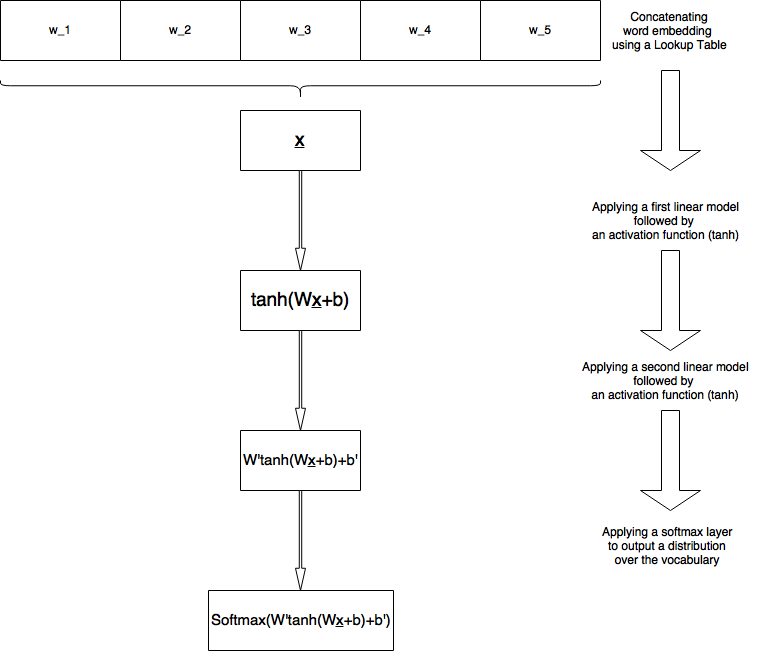
\includegraphics[width=0.4\textwidth]{reg.png}
    \caption{\underline{Neural Language Model (Bengio,2003)}}
\end{center}
\end{figure}

We then implemented a variant of the model using a skip-layer that concatenates the output of the tanh layer again with the original embeddings. The updated formula for the model is:

$$ nnlm_2(\boldsymbol{x}) = [\tanh(\boldsymbol{xW}+\boldsymbol{b}),\boldsymbol{x}]\boldsymbol{W'}+\boldsymbol{b'}$$

where this time:
\begin{itemize}
\item $\boldsymbol{W'}\in \Re^{(d_{hid}+ d_{in}\cdot d_{win})\times |\mathcal{V}|}$, and $\boldsymbol{b'}\in \Re^{|\mathcal{V}|}$
\end{itemize}

The updated diagram is as follows:
\begin{figure}[H]
\begin{center}
    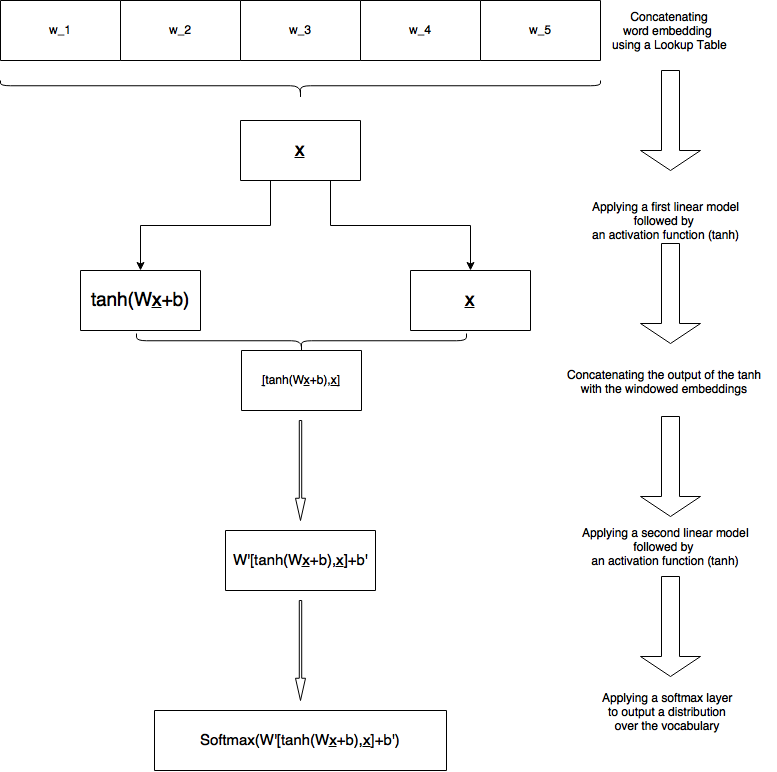
\includegraphics[width=0.5\textwidth]{skip.png}
    \caption{\underline{Skip-Layer Model}}
\end{center}
\end{figure}

We now show the pseudo code for training these NNLM using batch stochastic gradient descent:
  \begin{algorithmic}[1]
    \Procedure{$NNLM_i$}{$win_{1},...,win_{n}$,MaxEpoch,BatchSize,LearningRate}
    \For{epoch = 1,MaxEpoch}
    \For{batch = 1, $|$train$|$/BatchSize}
    \For{win in batch}
    \State{Call $NNLM_i$:forward(win)}
    \State{Evalute the loss}
    \State{Evaluate derivatives of the loss}
    \State{Backprop through $NNLM_i$}
    \EndFor{}
    \State{Update Parameters with LearningRate}
    \EndFor{}
    
    \EndFor{}
    \EndProcedure{}
  \end{algorithmic}


\subsubsection{Noise Contrastive Estimation}



\section{Experiments}

We now present the results of our experiments. We will first talk about the preprocessing and then continue with a comparison of the different models.

\subsection{Data and Preprocessing}

To complete this homework, we were given 3 datasets, one for training, one for validation and one for testing. The train set consisted of sentences with a total of over eight hundred thousands words from a vocabulary of ten thousands words. The validation set consisted of 70391 words. The particularity of the issue at hand consisted in the fact that we had to only predict a probability distribution over 50 words and not on the entire vocabulary. This is why we were provided the same validation set in the same format as for the test set. We could therefore predict 3370 words on the validation set to help us predict the 3361 words of the test set.\\

\noindent Most of the preprocessing was about building the N-grams for the different sets. We included in the preprocess.py file different functions to evaluate the windows as well as counting the different occurences of each N-grams. For instance, looking at 6-grams gave:

\begin{itemize}
\item 772 670 unique 6-grams on the training set,
\item 887 522 6-grams in total,
\item 70 391 6-grams on the validation set,
\item 3 370 words to predict on the validation set,
\item and 3 361 words of the test set
\end{itemize}

\subsection{Count-based Models}

\subsection{Neural Models}

The main issue we faced with Bengio's model was training time. Even we managed to have a working model with a smaller vocabulary, we struggled at first to get a code that ran fast enough to experiment extensively with different paremetrisations. Our original code ran one epoch in about one hour for the paremetrisation. While trying to code the NCE approximation, we nevertheless managed to cut the training time to about 14-15 minutes.\\

We decided to train the more complex neural network i.e. the one with the skip-layer, with the parametrisation suggested by Bengio:

\begin{itemize}
\item Window size: $d_{win} = 5$
\item Dimension of the embeddings: $d_{in} = 30$
\item Hidden dimension: $d_{hid} = 100$
\end{itemize}

We summarize the results in the graphs below:
\subsection{NCE}

We unfortunately did not succeed to implement a valid version of the Noise Contrastive Estimation. We did not managed to have a speed improvement and even worse observed that the perplexity on the validation was increasing instead of decreasing.

\section{Conclusion}

End the write-up with a very short recap of the main experiments and the main results. Describe any challenges you may have faced, and what could have been improved in the model.

\bibliographystyle{apalike}
\bibliography{writeup}

\end{document}
